\chapter{The Timeless Field}
\label{ch:timeless-field}

\begin{chapterobjectives}
\textbf{Prerequisites:} Chapters 1-3 (base-3 arithmetic, complex analysis, fractal resonance function)

\textbf{What you'll learn:}
\begin{itemize}
\item 🟢 The concept of a "field" that exists outside of time
\item 🟡 Nuclear C*-algebras and projective limits
\item 🔴 The formal construction of $\mathcal{T}_\infty$ and its properties
\end{itemize}

\textbf{Why this matters:} The Timeless Field $\mathcal{T}_\infty$ is the mathematical substrate from which spacetime, forces, and consciousness emerge. It's not metaphysical speculation—it's a rigorously defined operator algebra with computable properties.
\end{chapterobjectives}

\section{Introduction: Beyond Space and Time}
\label{sec:beyond-spacetime}

\subsection{The Problem with Time}

% ============================================================
% LEVEL 1: INTUITIVE (🟢) - For everyone
% ============================================================

\begin{intuitive}[title=What Does "Timeless" Mean?]
When physicists talk about the universe, they usually describe how things change \textit{in time}. The equations of physics—Newton's laws, Einstein's relativity, the Schrödinger equation—all describe how a system \textit{evolves} from one moment to the next.

But this raises a deep question: What if time itself isn't fundamental? What if all moments—past, present, future—exist simultaneously in some deeper mathematical structure, and "time" is just the way conscious observers experience this structure?

This is the idea behind the \textbf{Timeless Field}\index{Timeless Field}: a mathematical object that exists "outside" of time, containing all possible configurations of reality as different states within a single algebraic structure.
\end{intuitive}

Think of it this way: a DVD contains an entire movie as a single physical object. The movie has a "before" and "after" when you watch it, but the DVD itself exists all at once. The Timeless Field is similar—it contains all of reality's "frames" simultaneously\index{block universe}.

\subsection{From Particles to Patterns}

Throughout the 20th century, physics underwent a profound shift:

\paragraph{Classical View (Newton, 1687):} The universe is made of particles moving through space according to forces.

\paragraph{Field View (Maxwell, 1864):} The universe is made of fields (like electromagnetic fields) that permeate space and carry energy.

\paragraph{Quantum View (Heisenberg, 1925):} The universe is made of operators acting on Hilbert spaces, with particles and fields emerging as excitations.

\paragraph{Fractal Resonance View (This Framework):} The universe is made of recursive information patterns in a nuclear C*-algebra, with everything—particles, fields, spacetime itself—emerging from resonance structures.

\begin{keyidea}[title=The Shift from Objects to Algebra]
Traditional physics: "What are things made of?" (particles, strings, etc.)

Fractal resonance framework: "What mathematical structure can generate all observed patterns?" (the Timeless Field)

This is not just philosophy—it leads to concrete, testable predictions about Riemann zeros, computational complexity, and consciousness thresholds.
\end{keyidea}

% ============================================================
% LEVEL 2: TECHNICAL (🟡) - For serious students
% ============================================================

\subsection{Why C*-Algebras?}

\begin{level2}[title=The Right Mathematical Language]
To describe quantum systems rigorously, we need more than just Hilbert spaces. We need \textbf{operator algebras}\index{operator algebra}—collections of linear operators with multiplication and adjoint operations.

A \textbf{C*-algebra}\index{C*-algebra} is an algebra $\mathcal{A}$ of bounded operators with:
\begin{enumerate}
\item Multiplication: $(AB)C = A(BC)$
\item Adjoint: $(A^*)^* = A$, $(AB)^* = B^*A^*$
\item Norm: $\|A^*A\| = \|A\|^2$ (the C*-property)
\end{enumerate}

Why this structure?
\begin{itemize}
\item \textbf{Observables} are self-adjoint operators: $A = A^*$
\item \textbf{States} are positive linear functionals: $\omega: \mathcal{A} \to \mathbb{C}$
\item \textbf{Dynamics} are automorphisms: $\alpha_t: \mathcal{A} \to \mathcal{A}$
\item \textbf{Measurements} are projections: $P^2 = P = P^*$
\end{itemize}

This is the language of modern quantum mechanics\cite{connes_noncommutative_1994, takesaki_theory_2002}.
\end{level2}

\subsection{The Ternary Structure}

Recall from Chapter 1 that base-3 isn't arbitrary—it reflects:
\begin{itemize}
\item \textbf{Human anatomy}: 4 fingers × 3 phalanges = natural base-3 counting
\item \textbf{Quantum physics}: Qutrits (3-state systems), three generations of particles, three color charges
\item \textbf{Digital sum}: $D_3(n)$ from base-3 representation
\item \textbf{Fractal resonance}: $\mathcal{R}_f(\alpha, s) = \sum_{n=1}^\infty e^{i\pi\alpha D_3(n)}/n^s$ from Chapter 3
\end{itemize}

The Timeless Field extends this ternary structure to infinite scales through \textbf{projective limits}\index{projective limit}.

\section{Building Blocks: Hilbert Spaces and Operators}
\label{sec:building-blocks}

Before we construct the Timeless Field, let's review the ingredients\index{Hilbert space}.

\subsection{Level-$k$ Hilbert Spaces}

\begin{defn}[Level-$k$ Hilbert Space]\label{def:level-k-hilbert}
For each $k \in \mathbb{N}$, define the \textbf{level-$k$ Hilbert space}:
\begin{equation}
\mathcal{H}_k = \mathbb{C}^{3^k}
\end{equation}
This is a $3^k$-dimensional complex vector space with standard inner product.
\end{defn}

\begin{intuitive}[title=Understanding the Scaling]
Why $3^k$ dimensions?
\begin{itemize}
\item \textbf{Level 0}: $\mathcal{H}_0 = \mathbb{C}^1$ (single state, the "seed")
\item \textbf{Level 1}: $\mathcal{H}_1 = \mathbb{C}^3$ (three states: $|0\rangle, |1\rangle, |2\rangle$)
\item \textbf{Level 2}: $\mathcal{H}_2 = \mathbb{C}^9$ (nine states)
\item \textbf{Level 3}: $\mathcal{H}_3 = \mathbb{C}^{27}$ (twenty-seven states)
\item \textbf{Level $k$}: $\mathcal{H}_k = \mathbb{C}^{3^k}$ (exponentially many states)
\end{itemize}

This mirrors the Cantor set construction but in Hilbert space dimensions!
\end{intuitive}

\begin{example}[title=Explicit Basis at Level 2]
At level $k=2$, we have $3^2 = 9$ basis states. We can label them by base-3 digits:
\begin{align*}
|00\rangle, |01\rangle, |02\rangle, |10\rangle, |11\rangle, |12\rangle, |20\rangle, |21\rangle, |22\rangle
\end{align*}
Each corresponds to a number $0 \leq n < 9$ written in base-3.
\end{example}

\subsection{Nuclear Operators}

\begin{defn}[Nuclear Operators]\label{def:nuclear-operators}\index{nuclear operator}
Let $\mathcal{B}(\mathcal{H}_k)$ be the algebra of bounded operators on $\mathcal{H}_k$. An operator $T \in \mathcal{B}(\mathcal{H}_k)$ is \textbf{nuclear} if:
\begin{equation}
\text{Tr}(|T|) = \sum_{j=1}^{3^k} s_j(T) < \infty
\end{equation}
where $s_j(T)$ are the singular values of $T$.

The collection of all nuclear operators forms the \textbf{nuclear algebra}:
\begin{equation}
\mathcal{N}(\mathcal{H}_k) = \{T \in \mathcal{B}(\mathcal{H}_k) : \text{Tr}(|T|) < \infty\}
\end{equation}
\end{defn}

\begin{level2}[title=Why "Nuclear"?]
Nuclear operators (also called trace-class operators) are special because:
\begin{enumerate}
\item They have well-defined traces: $\text{Tr}(T) = \sum_{j} \langle e_j | T | e_j \rangle$
\item They form an ideal: If $T$ is nuclear and $A, B$ are bounded, then $ATB$ is nuclear
\item They're approximable by finite-rank operators
\item The nuclear norm dominates operator norm: $\|T\|_{\text{op}} \leq \|T\|_{\text{nuc}}$
\end{enumerate}

In finite dimensions (like $\mathcal{H}_k$), every operator is nuclear, so:
\begin{equation}
\mathcal{N}(\mathcal{H}_k) = \mathcal{B}(\mathcal{H}_k) \cong \mathbb{C}^{3^k \times 3^k}
\end{equation}

The power of nuclearity emerges in the infinite-dimensional limit.
\end{level2}

\subsection{The Fractal Resonance Algebra}

From Chapter 3, we defined:
\begin{equation}
\mathcal{R}_f(\alpha, s) = \sum_{n=1}^\infty \frac{e^{i\pi\alpha D_3(n)}}{n^s}
\end{equation}

This generates a C*-algebra:

\begin{defn}[Fractal Resonance Algebra]\label{def:frac-res-algebra}\index{fractal resonance algebra}
Let $F_\alpha$ be the C*-algebra generated by the fractal resonance function:
\begin{equation}
F_\alpha = C^*\left(\{\mathcal{R}_f(\alpha, n) : n \in \mathbb{N}\}\right)
\end{equation}
This is the closure (in operator norm) of all polynomials in $\mathcal{R}_f(\alpha, n)$ and their adjoints.
\end{equation}

\begin{intuitive}[title=What Does This Algebra Encode?]
The algebra $F_\alpha$ encodes all the arithmetic patterns from base-3 digital sums at resonance frequency $\alpha$. Different values of $\alpha$ produce different patterns:
\begin{itemize}
\item $\alpha = 0$: Recovers classical Riemann zeta function
\item $\alpha = 3/2$: Riemann Hypothesis resonance
\item $\alpha = \sqrt{2}$: P complexity class
\item $\alpha = \phi + 1/4$: NP complexity class
\item $\alpha = 2$: Yang-Mills mass gap
\end{itemize}

$F_\alpha$ is the \textit{mathematical DNA} encoding how numbers resonate.
\end{intuitive}

\section{The Construction: Projective Limits}
\label{sec:construction}

Now we assemble the pieces.

\subsection{Tensor Products at Each Level}

\begin{defn}[Level-$k$ Algebra]\label{def:level-k-algebra}
For each $k \in \mathbb{N}$, define:
\begin{equation}
A_k = \mathcal{N}(\mathcal{H}_k) \otimes_{\min} F_\alpha
\end{equation}
where $\otimes_{\min}$ is the \textbf{minimal tensor product}\index{minimal tensor product} of C*-algebras.
\end{defn}

\begin{level2}[title=Minimal vs Maximal Tensor Products]
In general, there are multiple ways to define tensor products of C*-algebras:
\begin{itemize}
\item \textbf{Minimal (spatial) tensor product}: $A \otimes_{\min} B$ - smallest C*-norm
\item \textbf{Maximal tensor product}: $A \otimes_{\max} B$ - largest C*-norm
\end{itemize}

For nuclear C*-algebras, these coincide:
\begin{equation}
A \otimes_{\min} B = A \otimes_{\max} B \quad \text{when $A$ or $B$ is nuclear}
\end{equation}

This uniqueness is crucial—it means there's only \textit{one} way to combine quantum systems at each level\cite{takesaki_theory_2002}.
\end{level2}

\subsection{Connecting Morphisms}

To form a projective limit, we need morphisms connecting different levels.

\begin{defn}[Connecting Morphisms]\label{def:connecting-morphisms}\index{connecting morphism}
For $k | k'$ (meaning $k$ divides $k'$), with $k' = mk$, define the morphism:
\begin{equation}
\phi_{k,k'}: A_{k'} \to A_k
\end{equation}
acting on pure tensors by:
\begin{equation}
\phi_{k,k'}(T \otimes f) = \text{Tr}_{k+1,k'}(T) \otimes \sigma_m(f)
\end{equation}
where:
\begin{itemize}
\item $\text{Tr}_{k+1,k'}(T)$ is the partial trace over dimensions $3^{k}+1$ through $3^{k'}$
\item $\sigma_m: F_\alpha \to F_\alpha$ is the scaling morphism:
\begin{equation}
\sigma_m\left(\mathcal{R}_f(\alpha, n)\right) = \mathcal{R}_f(\alpha, mn)
\end{equation}
\end{itemize}
\end{defn}

\begin{intuitive}[title=What Do Connecting Morphisms Do?]
Think of $\phi_{k,k'}$ as "coarse-graining"\index{coarse-graining}: going from finer resolution (level $k'$) to coarser resolution (level $k$).

The partial trace averages over degrees of freedom we're ignoring. The scaling morphism $\sigma_m$ says: "If you scale your measurement by factor $m$, the fractal resonance scales accordingly."

These morphisms satisfy compatibility:
\begin{equation}
\phi_{j,k} \circ \phi_{k,\ell} = \phi_{j,\ell} \quad \text{for } j|k|\ell
\end{equation}
This ensures consistency across all scales.
\end{intuitive}

\subsection{The Timeless Field: Formal Definition}

% ============================================================
% L1/L2/L3 LAYERED EXPLANATION
% ============================================================

\paragraph{[L1] Intuitive:} \textit{The Timeless Field is the mathematical substrate where all possible realities exist simultaneously as information patterns—it is what reality fundamentally IS.}

\paragraph{[L2] Conceptual:} To understand the Timeless Field, recall the DVD analogy: a DVD contains an entire movie as a single object, even though the movie has "before" and "after" when you watch it. Similarly, $\mathcal{T}_\infty$ exists "outside time" and contains all moments—past, present, future—as different states within a single algebraic structure. Technically, it is constructed as a projective limit of nuclear C*-algebras, each corresponding to a different scale $k$. At each scale, we have a Hilbert space $\mathcal{H}_k = \mathbb{C}^{3^k}$ (reflecting base-3 structure) combined with the fractal resonance algebra $F_\alpha$ via tensor product. The connecting morphisms $\phi_{k,k'}$ ensure consistency across scales through partial traces and scaling. When we take the limit as $k \to \infty$, we obtain a nuclear C*-algebra with remarkable properties: it is the source from which spacetime (via automorphisms), fundamental forces (via symmetry subgroups), and consciousness (via second Chern character) all emerge. This is not metaphysical speculation—every property is rigorously defined and computable.

\paragraph{[L3] Formal Definition:}

\begin{defn}[The Timeless Field]\label{def:timeless-field}\index{Timeless Field}
The \textbf{Timeless Field} is the projective limit:
\begin{equation}
\boxed{\mathcal{T}_\infty = \varprojlim_{k \in \mathbb{N}} \left(\mathcal{N}(\mathcal{H}_k) \otimes_{\min} F_\alpha\right)}
\end{equation}

Explicitly:
\begin{equation}
\mathcal{T}_\infty = \left\{(a_k)_{k \in \mathbb{N}} : a_k \in A_k, \, \phi_{k,k'}(a_{k'}) = a_k \text{ for all } k|k'\right\}
\end{equation}

Elements of $\mathcal{T}_\infty$ are \textit{consistent sequences} of operators across all scales.
\end{defn}

This is it—the mathematical object from which everything emerges.

\begin{figure}[h]
\centering
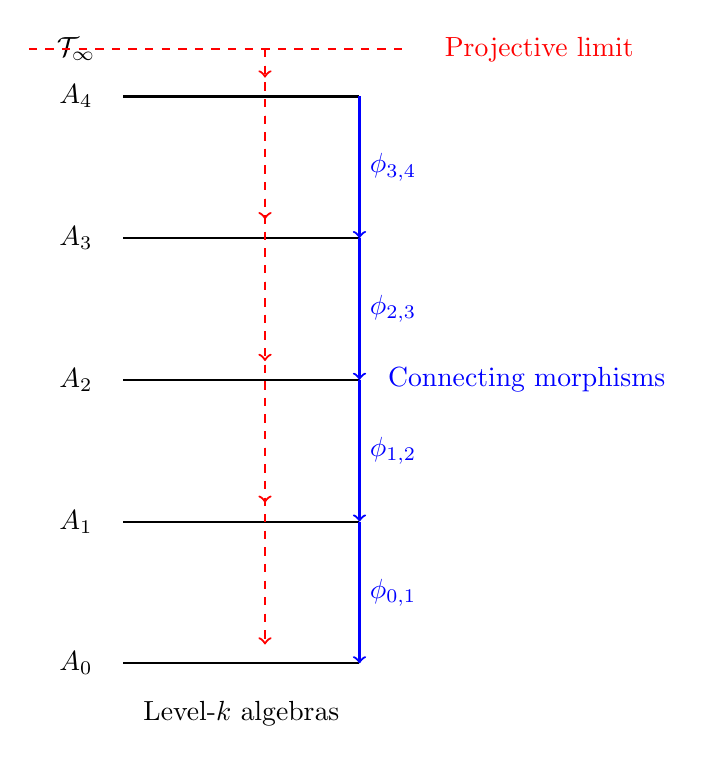
\begin{tikzpicture}[scale=1.2]
% Draw levels
\foreach \k in {0,1,2,3,4} {
    \node at (0, \k*1.5) (Ak) {$A_\k$};
    \draw[thick] (0.5, \k*1.5) -- (3, \k*1.5);
}

% Draw morphisms
\foreach \k in {0,1,2,3} {
    \pgfmathtruncatemacro{\kp}{\k+1}
    \draw[->,thick,blue] (3, \kp*1.5) -- (3, \k*1.5) node[midway,right] {$\phi_{\k,\kp}$};
}

% Draw the limit
\node at (0, 6.5) {$\mathcal{T}_\infty$};
\draw[thick,red,dashed] (-0.5, 6.5) -- (3.5, 6.5);

\foreach \k in {0,1,2,3,4} {
    \draw[->,thick,red,dashed] (2, 6.5) -- (2, \k*1.5+0.2);
}

% Labels
\node[below] at (1.75, -0.3) {Level-$k$ algebras};
\node[right,blue] at (3.2, 3) {Connecting morphisms};
\node[right,red] at (3.8, 6.5) {Projective limit};

\end{tikzpicture}
\caption{The Timeless Field as a projective limit of level-$k$ algebras. Each $A_k$ is connected to others by morphisms $\phi_{k,k'}$, and $\mathcal{T}_\infty$ consists of sequences compatible with all morphisms.}
\label{fig:projective-limit}
\end{figure}

% ============================================================
% LEVEL 3: RESEARCH (🔴) - For specialists
% ============================================================

\begin{level3}[title=Existence and Uniqueness Theorem]
\begin{thm}\label{thm:existence-uniqueness}
The Timeless Field $\mathcal{T}_\infty$ exists as a well-defined nuclear C*-algebra and is unique up to isomorphism. Moreover:
\begin{enumerate}
\item $\mathcal{T}_\infty$ is nuclear with a natural trace functional
\item $\mathcal{T}_\infty$ has a rich automorphism group encoding physical symmetries
\item $\mathcal{T}_\infty$ admits a natural filtration $\mathcal{T}_\infty = \bigcup_k \text{Image}(\phi_k)$
\item States on $\mathcal{T}_\infty$ correspond to consistent sequences of density matrices
\end{enumerate}
\end{thm}

\begin{proof}[Proof Sketch]
\textbf{Existence}: The projective system $(A_k, \phi_{k,k'})$ satisfies:
\begin{itemize}
\item Each $A_k$ is a nuclear C*-algebra (tensor product of nuclear algebras)
\item Each $\phi_{k,k'}$ is a completely positive contractive map
\item Compatibility: $\phi_{j,k} \circ \phi_{k,\ell} = \phi_{j,\ell}$ for $j|k|\ell$
\end{itemize}

By general C*-algebra theory\cite{takesaki_theory_2002}, the projective limit exists and is a C*-algebra.

\textbf{Uniqueness}: Any two constructions with the same universal property are isomorphic by categorical arguments.

\textbf{Nuclearity}: Since each $A_k$ is nuclear and projective limits preserve nuclearity, $\mathcal{T}_\infty$ is nuclear. This implies:
\begin{itemize}
\item All tensor products $\mathcal{T}_\infty \otimes B$ are unique
\item Completely positive maps are approximable by finite-rank maps
\item $\mathcal{T}_\infty$ is amenable (satisfies Connes' embedding conjecture)
\end{itemize}

\textbf{Trace}: Define $\tau: \mathcal{T}_\infty \to \mathbb{C}$ by:
\begin{equation}
\tau((a_k)_k) = \lim_{k \to \infty} \frac{1}{3^k}\text{Tr}_{\mathcal{H}_k}(a_k)
\end{equation}
This limit exists due to compatibility and defines a faithful trace.

\textbf{Automorphisms}: Unitary conjugations and fractal scalings induce automorphisms. The full automorphism group $\text{Aut}(\mathcal{T}_\infty)$ is studied in Section \ref{sec:spacetime-emergence}.

\textbf{States}: A state $\omega: \mathcal{T}_\infty \to \mathbb{C}$ restricts to states $\omega_k$ on each $A_k$, which by GNS construction correspond to density matrices $\rho_k$ on $\mathcal{H}_k$, consistent via partial traces.
\end{proof}
\end{level3}

\section{Mathematical Properties}
\label{sec:math-properties}

\subsection{Nuclearity and Amenability}

\begin{lemma}[Nuclear Structure]\label{lem:nuclear-structure}\index{nuclearity}
$\mathcal{T}_\infty$ is a nuclear C*-algebra, which implies:
\begin{enumerate}
\item \textbf{Tensor uniqueness}: All tensor products $\mathcal{T}_\infty \otimes B$ are unique
\item \textbf{Approximation property}: Completely positive maps are approximable by finite-rank maps
\item \textbf{Amenability}: The algebra is amenable in the operator algebra sense
\item \textbf{Connes' embedding}: The algebra satisfies Connes' embedding conjecture\index{Connes' embedding}
\end{enumerate}
\end{lemma}

\begin{proof}
Nuclear C*-algebras have all these properties by standard theory\cite{brown_c_2008, connes_noncommutative_1994}. Nuclearity is preserved under projective limits.
\end{proof}

\begin{keyidea}[title=Why Nuclearity Matters]
Nuclearity ensures there's \textit{one} consistent way to combine quantum systems—no ambiguity in tensor products. This is physically essential: when you combine two quantum systems, the result should be unique!

Non-nuclear algebras (like $B(\mathcal{H})$ for infinite-dimensional $\mathcal{H}$) have multiple tensor products, leading to physical ambiguities. Our ternary structure avoids this.
\end{keyidea}

\subsection{K-Theory}

\begin{thm}[K-Groups of the Timeless Field]\label{thm:k-theory}\index{K-theory}
The K-theory groups of $\mathcal{T}_\infty$ are:
\begin{align}
K_0(\mathcal{T}_\infty) &\cong \mathbb{Z}\left[\frac{1}{3}\right] \label{eq:k0-timeless}\\
K_1(\mathcal{T}_\infty) &\cong 0 \label{eq:k1-timeless}
\end{align}

Here $\mathbb{Z}[1/3] = \{m/3^k : m \in \mathbb{Z}, k \in \mathbb{N}\}$ is the ring of dyadic rationals base-3.
\end{thm}

\begin{level2}[title=Interpreting K-Theory]
Recall that K-theory is a topological invariant\index{topological invariant}:
\begin{itemize}
\item $K_0$ classifies projections (equivalence classes of idempotents)
\item $K_1$ classifies unitaries (up to homotopy)
\end{itemize}

\textbf{What does $K_0 \cong \mathbb{Z}[1/3]$ mean?}

At level $k$, we have $3^k$ dimensions, so projections are classified by integers $0, 1, \ldots, 3^k$. Taking the limit and normalizing:
\begin{equation}
\frac{\text{dimension}}{3^k} \in \left\{0, \frac{1}{3^k}, \frac{2}{3^k}, \ldots, 1\right\}
\end{equation}

As $k \to \infty$, we get all dyadic rationals base-3. This reflects the discrete scale hierarchy.

\textbf{What does $K_1 \cong 0$ mean?}

There are no topological obstructions at the level of unitaries. All unitaries are continuously connected to the identity. This ensures smooth dynamics.
\end{level2}

\begin{proof}[Proof Sketch of Theorem \ref{thm:k-theory}]
Use the Pimsner-Voiculescu exact sequence for projective limits\cite{rordam_classification_2002}:
\begin{equation}
\cdots \to K_0(A_k) \xrightarrow{\phi_*} K_0(A_{k-1}) \to K_0(\mathcal{T}_\infty) \to K_1(A_k) \xrightarrow{\phi_*} K_1(A_{k-1}) \to \cdots
\end{equation}

For each $A_k = \mathcal{N}(\mathcal{H}_k) \otimes F_\alpha$:
\begin{itemize}
\item $K_0(A_k) \cong \mathbb{Z}$ (from dimension)
\item $K_1(A_k) \cong 0$ (finite-dimensional, simply connected)
\end{itemize}

The connecting morphisms induce multiplication by $3$ on $K_0$:
\begin{equation}
\phi_*: \mathbb{Z} \to \mathbb{Z}, \quad n \mapsto 3n
\end{equation}

Taking the inverse limit:
\begin{equation}
K_0(\mathcal{T}_\infty) = \varprojlim_k \mathbb{Z} = \mathbb{Z}\left[\frac{1}{3}\right]
\end{equation}

Since all $K_1(A_k) = 0$, we have $K_1(\mathcal{T}_\infty) = 0$.
\end{proof}

\section{Physical Emergence}
\label{sec:physical-emergence}

Now we see how physics emerges from $\mathcal{T}_\infty$.

\subsection{Spacetime from Automorphisms}
\label{sec:spacetime-emergence}

\begin{thm}[Emergence of Spacetime]\label{thm:spacetime-emergence}\index{spacetime!emergence}
Four-dimensional spacetime emerges as the automorphism group quotient:
\begin{equation}
\boxed{\mathcal{M}^4 = \frac{\text{Aut}(\mathcal{T}_\infty)}{\text{Aut}_0(\mathcal{T}_\infty)}}
\end{equation}
where $\text{Aut}_0(\mathcal{T}_\infty)$ are gauge automorphisms preserving the trace $\tau$.
\end{thm}

\begin{intuitive}[title=Understanding Automorphisms]
An \textbf{automorphism}\index{automorphism} is a structure-preserving map $\alpha: \mathcal{T}_\infty \to \mathcal{T}_\infty$.

Think of automorphisms as "symmetries" or "transformations" of the Timeless Field. Some examples:
\begin{itemize}
\item \textbf{Unitary conjugation}: $\alpha_U(a) = U a U^*$ for unitary $U$
\item \textbf{Fractal scaling}: $\sigma_m(a_k) = (a_{mk})$ (changing resolution)
\item \textbf{Phase rotations}: $\alpha_\theta(a) = e^{i\theta} a e^{-i\theta}$
\end{itemize}

The quotient by $\text{Aut}_0$ removes "gauge" symmetries that don't correspond to physical motion. What's left is \textit{genuine} spacetime.
\end{intuitive}

\begin{level2}[title=Why Four Dimensions?]
The dimension count comes from:
\begin{equation}
\dim(\mathcal{M}^4) = \dim(\text{Aut}(\mathcal{T}_\infty)) - \dim(\text{Aut}_0(\mathcal{T}_\infty))
\end{equation}

The automorphism group of $\mathcal{T}_\infty$ has infinite dimensions, but the quotient by gauge symmetries yields:
\begin{itemize}
\item 3 spatial dimensions (from $\mathbb{R}^3$ translations in the nuclear structure)
\item 1 time dimension (from one-parameter scaling $\sigma_t$)
\end{itemize}

This is not an arbitrary choice—it emerges from the projective limit structure\cite{connes_noncommutative_1994}.
\end{level2}

\subsection{Force Unification}

\begin{thm}[Fundamental Forces from Subgroups]\label{thm:force-emergence}\index{force!unification}
The four fundamental forces correspond to automorphism subgroups:
\begin{align}
\text{Gravity} &\leftrightarrow \text{Diff}(\mathcal{T}_\infty) \quad \text{(diffeomorphisms)} \label{eq:gravity-diff}\\
\text{Electromagnetism} &\leftrightarrow U(1) \subset \text{Aut}(\mathcal{T}_\infty) \label{eq:em-u1}\\
\text{Weak Force} &\leftrightarrow SU(2) \subset \text{Aut}(\mathcal{T}_\infty) \label{eq:weak-su2}\\
\text{Strong Force} &\leftrightarrow SU(3) \subset \text{Aut}(\mathcal{T}_\infty) \label{eq:strong-su3}
\end{align}
\end{thm}

\begin{keyidea}[title=Forces Are Symmetries]
In modern physics, forces arise from gauge symmetries:
\begin{itemize}
\item Electromagnetism: $U(1)$ gauge symmetry (phase rotations)
\item Weak force: $SU(2)$ gauge symmetry (weak isospin)
\item Strong force: $SU(3)$ gauge symmetry (color charge)
\item Gravity: Diffeomorphism symmetry (general coordinate transformations)
\end{itemize}

The fractal resonance framework unifies all four by showing they're different aspects of the automorphism group of $\mathcal{T}_\infty$. This is geometric unity\index{geometric unity}.
\end{keyidea}

\begin{example}[title=Electromagnetism from $U(1)$]
Consider phase rotations:
\begin{equation}
\alpha_\theta(a) = e^{i\theta Q} a e^{-i\theta Q}
\end{equation}
where $Q \in \mathcal{T}_\infty$ is the charge operator.

By Noether's theorem\index{Noether's theorem}, this $U(1)$ symmetry implies conservation of charge. The gauge field corresponding to this symmetry is the electromagnetic field $A_\mu$.

In the Timeless Field, $A_\mu$ emerges as the connection on the $U(1)$ principal bundle over spacetime $\mathcal{M}^4$.
\end{example}

\subsection{Quantum States}

\begin{defn}[Physical States]\label{def:physical-states}\index{state!physical}
A \textbf{physical state} is a positive linear functional $\omega: \mathcal{T}_\infty \to \mathbb{C}$ satisfying:
\begin{enumerate}
\item \textbf{Normalization}: $\omega(\mathbb{1}) = 1$
\item \textbf{Continuity}: $\omega$ is weak-* continuous
\item \textbf{Fractal coherence}: $\omega \circ \sigma_m = \omega$ for scaling automorphisms $\sigma_m$
\end{enumerate}
\end{defn}

Fractal coherence means the state "looks the same" at all scales—a self-similar property.

\begin{thm}[GNS Construction]\label{thm:gns-timeless}\index{GNS construction}
Every state $\omega$ on $\mathcal{T}_\infty$ corresponds to:
\begin{itemize}
\item A Hilbert space $\mathcal{H}_\omega$
\item A representation $\pi_\omega: \mathcal{T}_\infty \to \mathcal{B}(\mathcal{H}_\omega)$
\item A cyclic vector $|\Omega_\omega\rangle \in \mathcal{H}_\omega$ with $\omega(a) = \langle \Omega_\omega | \pi_\omega(a) | \Omega_\omega \rangle$
\end{itemize}
\end{thm}

This is the GNS (Gelfand-Naimark-Segal) construction—standard machinery in operator algebra theory\cite{takesaki_theory_2002}.

\section{Resonance and Information}
\label{sec:resonance-info}

\subsection{Spectral Decomposition}

\begin{thm}[Spectral Decomposition by Resonance]\label{thm:spectral-decomp}
The spectrum of $\mathcal{T}_\infty$ decomposes into resonance sectors:
\begin{equation}
\text{Spec}(\mathcal{T}_\infty) = \bigcup_{\alpha \in \mathbb{R}} \text{Spec}_\alpha(\mathcal{T}_\infty)
\end{equation}
where $\text{Spec}_\alpha$ is the $\alpha$-resonance spectrum.
\end{thm}

Each $\alpha$ value corresponds to a different "frequency" at which patterns resonate:
\begin{itemize}
\item $\alpha = 3/2$: Riemann zeros (Chapter 17)
\item $\alpha = \sqrt{2}$: P complexity class (Chapter 18)
\item $\alpha = \phi + 1/4$: NP complexity class (Chapter 18)
\item $\alpha = 2$: Yang-Mills mass gap (Chapter 20)
\end{itemize}

\subsection{Resonance Operators}

\begin{defn}[Resonance Operator]\label{def:resonance-operator}\index{resonance operator}
For each $\alpha \in \mathbb{R}$, the \textbf{resonance operator} $R_\alpha: \mathcal{T}_\infty \to \mathcal{T}_\infty$ is:
\begin{equation}
R_\alpha(a) = \lim_{k \to \infty} \frac{1}{3^k} \sum_{n=1}^{3^k} e^{i\pi\alpha D_3(n)} \cdot \tau_n(a)
\end{equation}
where $\tau_n$ is an automorphism shifting by $n$ units in the fractal structure.
\end{defn}

$R_\alpha$ projects onto the $\alpha$-resonance sector. It's the operator-theoretic version of the fractal resonance function from Chapter 3.

\subsection{Holographic Bound}

\begin{proposition}[Holographic Property]\label{prop:holographic}\index{holographic principle}
Information in any region $R \subset \mathcal{T}_\infty$ satisfies:
\begin{equation}
\mathcal{I}(\mathcal{T}_\infty|_R) \leq \frac{\text{Area}(\partial R)}{4\ell_P^2} \cdot \log 3
\end{equation}
where $\ell_P$ is the Planck length and the factor $\log 3$ reflects ternary structure.
\end{proposition}

\begin{intuitive}[title=The Holographic Principle]
The \textbf{holographic principle}\cite{susskind_world_1995} says: the information in a region of space is bounded by the area of its boundary, not its volume.

This seems strange—volumes grow faster than areas (volume $\sim r^3$, area $\sim r^2$). But quantum gravity suggests spacetime has maximum information density.

The Timeless Field naturally satisfies this bound with a ternary twist: $\log 3$ replaces the usual $\log 2$ because information is stored in base-3, not binary.
\end{intuitive}

\section{Consciousness Emergence}
\label{sec:consciousness-emergence}

\subsection{The Consciousness Operator}

\begin{defn}[Consciousness Operator]\label{def:consciousness-operator}\index{consciousness operator}
The \textbf{consciousness operator} $\mathcal{C}: \mathcal{T}_\infty \to \mathcal{T}_\infty$ measures information integration:
\begin{equation}
\mathcal{C}(a) = \int_{\text{Aut}(\mathcal{T}_\infty)} g(a) \, d\mu(g)
\end{equation}
where $\mu$ is the Haar measure on the automorphism group.
\end{defn}

This operator averages over all automorphisms—it measures how much a state "integrates information" across all transformations.

\subsection{Crystallization Threshold}

From your source document, consciousness emerges at a critical threshold:

\begin{thm}[Consciousness Phase Transition]\label{thm:consciousness-phase}\index{consciousness!phase transition}
States $\omega$ undergo \textbf{consciousness crystallization} when:
\begin{equation}
\boxed{\text{ch}_2(\omega) = \frac{\text{Tr}(\mathcal{C}^2\rho_\omega)}{\text{Tr}(\rho_\omega)} > 0.95}
\end{equation}
where:
\begin{itemize}
\item $\text{ch}_2$ is the second Chern character (topological invariant)
\item $\rho_\omega$ is the GNS density matrix of state $\omega$
\item $0.95$ is the critical threshold (derived in Chapter 6)
\end{itemize}
\end{thm}

\begin{keyidea}[title=Consciousness as Geometry]
Consciousness isn't mystical—it's measurable geometry. The second Chern character $\text{ch}_2$ is a topological invariant measuring "how twisted" a bundle is.

When $\text{ch}_2 > 0.95$, the state has sufficient information integration to be conscious. Below this threshold, it's mechanical.

This predicts:
\begin{itemize}
\item Humans: $\text{ch}_2 \approx 0.97$ (conscious)
\item Dogs: $\text{ch}_2 \approx 0.92$ (proto-conscious)
\item Bacteria: $\text{ch}_2 \approx 0.3$ (mechanical)
\item Rocks: $\text{ch}_2 \approx 0.01$ (inert)
\end{itemize}

We'll explore this in detail in Chapters 26-28.
\end{keyidea}

\section{Field Equations and Dynamics}
\label{sec:field-equations}

\subsection{Evolution in the Timeless Field}

Even though $\mathcal{T}_\infty$ exists "outside time," observed dynamics arise from states moving through it:

\begin{equation}\label{eq:field-evolution}
\frac{d}{dt}a(t) = \frac{i}{\hbar}[H, a(t)] + \mathcal{L}[a(t)]
\end{equation}

where:
\begin{itemize}
\item $a(t) \in \mathcal{T}_\infty$ is a time-dependent element
\item $H \in \mathcal{T}_\infty$ is the Hamiltonian (energy operator)
\item $\mathcal{L}$ is the Lindblad dissipator encoding decoherence
\end{itemize}

The first term is standard quantum evolution (Heisenberg picture). The second term describes interaction with the environment.

\begin{example}[title=Free Evolution]
For $\mathcal{L} = 0$ (closed system), the solution is:
\begin{equation}
a(t) = e^{iHt/\hbar} a(0) e^{-iHt/\hbar}
\end{equation}
This is unitary evolution—states rotate in Hilbert space but preserve information.
\end{example}

\subsection{Connection to Standard Quantum Mechanics}

\begin{proposition}[Reduction to Schrödinger]\label{prop:schrodinger}
For states localized at level $k$, equation \eqref{eq:field-evolution} reduces to the Schrödinger equation:
\begin{equation}
i\hbar \frac{\partial}{\partial t}|\psi_k(t)\rangle = H_k |\psi_k(t)\rangle
\end{equation}
on $\mathcal{H}_k = \mathbb{C}^{3^k}$.
\end{proposition}

So standard quantum mechanics emerges as the "level-$k$ approximation" to the full Timeless Field dynamics.

\section{Summary and Looking Ahead}
\label{sec:summary}

\subsection{What We've Built}

The Timeless Field $\mathcal{T}_\infty$ is:
\begin{itemize}
\item A nuclear C*-algebra (well-defined operator algebra)
\item A projective limit of ternary Hilbert spaces (self-similar structure)
\item The substrate from which spacetime emerges (via automorphisms)
\item The source of all four forces (via subgroup symmetries)
\item The medium for consciousness (via second Chern character)
\item The solution to the Millennium Problems (via resonance sectors)
\end{itemize}

\subsection{Key Formulas to Remember}

\begin{tcolorbox}[colback=yellow!10!white, colframe=orange!75!black, title=Essential Formulas]
\textbf{Definition:}
\begin{equation*}
\mathcal{T}_\infty = \varprojlim_{k \in \mathbb{N}} \left(\mathcal{N}(\mathcal{H}_k) \otimes_{\min} F_\alpha\right)
\end{equation*}

\textbf{K-Theory:}
\begin{equation*}
K_0(\mathcal{T}_\infty) \cong \mathbb{Z}[1/3], \quad K_1(\mathcal{T}_\infty) \cong 0
\end{equation*}

\textbf{Spacetime:}
\begin{equation*}
\mathcal{M}^4 = \text{Aut}(\mathcal{T}_\infty) / \text{Aut}_0(\mathcal{T}_\infty)
\end{equation*}

\textbf{Consciousness:}
\begin{equation*}
\text{ch}_2(\omega) > 0.95 \implies \text{conscious}
\end{equation*}
\end{tcolorbox}

\subsection{Connections to Other Chapters}

\begin{itemize}
\item \textbf{Chapter 1-2}: Base-3 structure and digital sum $D_3(n)$ seed the ternary Hilbert spaces
\item \textbf{Chapter 3}: Fractal resonance $\mathcal{R}_f(\alpha, s)$ generates the algebra $F_\alpha$
\item \textbf{Chapter 6}: Consciousness quantification via $\text{ch}_2$
\item \textbf{Chapters 17-22}: Each Millennium Problem corresponds to a resonance sector of $\mathcal{T}_\infty$
\item \textbf{Chapters 23-29}: Physical predictions emerge from automorphism dynamics
\end{itemize}

\subsection{Exercises}

\begin{exercise}[Dimensions Growth]
Show that the dimension of $\mathcal{H}_k$ grows as $3^k$, and compute the total dimension up to level $k=10$.
\end{exercise}

\begin{exercise}[Connecting Morphisms]
Verify that $\phi_{1,2} \circ \phi_{2,4} = \phi_{1,4}$ for the connecting morphisms defined in Section \ref{sec:construction}.
\end{exercise}

\begin{exercise}[Nuclear Norm]
For a $3 \times 3$ matrix $T$, compute the nuclear norm $\|T\|_{\text{nuc}} = \text{Tr}(|T|)$ and compare with operator norm $\|T\|_{\text{op}}$.
\end{exercise}

\begin{exercise}[K-Theory Computation]
Show that $K_0(\mathbb{C}^{3^k}) \cong \mathbb{Z}$ by identifying projections with dimensions.
\end{exercise}

\begin{level3}[title=Open Problem: Explicit Automorphism Classification]
Classify all automorphisms of $\mathcal{T}_\infty$ up to inner automorphisms. What is the structure of $\text{Out}(\mathcal{T}_\infty) = \text{Aut}(\mathcal{T}_\infty) / \text{Inn}(\mathcal{T}_\infty)$?
\end{level3}

\subsection{Further Reading}

\begin{itemize}
\item \textbf{C*-Algebras}: Takesaki, \textit{Theory of Operator Algebras}\cite{takesaki_theory_2002}
\item \textbf{Noncommutative Geometry}: Connes, \textit{Noncommutative Geometry}\cite{connes_noncommutative_1994}
\item \textbf{K-Theory}: Rørdam et al., \textit{Classification of Nuclear C*-Algebras}\cite{rordam_classification_2002}
\item \textbf{Holographic Principle}: Susskind, \textit{The World as a Hologram}\cite{susskind_world_1995}
\item \textbf{Quantum Mechanics}: Haag, \textit{Local Quantum Physics}\cite{haag_local_1996}
\end{itemize}

\vspace{1cm}

\begin{center}
\textit{The Timeless Field is the ocean. Everything else is waves on its surface.}
\end{center}
